% --------------------------------------------------------------
% This is all preamble stuff that you don't have to worry about.
% Head down to where it says "Start here"
% --------------------------------------------------------------
 
\documentclass[12pt]{article}
 
\usepackage[margin=1in]{geometry} 
\usepackage{amsmath,amsthm,amssymb,scrextend}
\usepackage{fancyhdr}
\usepackage{enumitem}
\usepackage{amsmath}
\usepackage{amssymb}
\usepackage{textcomp}
\usepackage{fancybox}
\usepackage{tikz}
\usepackage{tasks}
\pagestyle{fancy}
\usepackage[makeroom]{cancel}
\usepackage{graphicx}
\usepackage{caption}
\usepackage{mwe}
\usepackage{tikz}
\usetikzlibrary{positioning}

\newcommand{\N}{\mathbb{N}}
\newcommand{\Z}{\mathbb{Z}}
\newcommand{\I}{\mathbb{I}}
\newcommand{\R}{\mathbb{R}}
\newcommand{\Q}{\mathbb{Q}}
\renewcommand{\qed}{\hfill$\blacksquare$}
\let\newproof\proof
\renewenvironment{proof}{\begin{addmargin}[1em]{0em}\begin{newproof}}{\end{newproof}\end{addmargin}\qed}
% \newcommand{\expl}[1]{\text{\hfill[#1]}$}
 
\newenvironment{theorem}[2][Theorem]{\begin{trivlist}
\item[\hskip \labelsep {\bfseries #1}\hskip \labelsep {\bfseries #2.}]}{\end{trivlist}}
\newenvironment{lemma}[2][Lemma]{\begin{trivlist}
\item[\hskip \labelsep {\bfseries #1}\hskip \labelsep {\bfseries #2.}]}{\end{trivlist}}
\newenvironment{problem}[2][Problem]{\begin{trivlist}
\item[\hskip \labelsep {\bfseries #1}\hskip \labelsep {\bfseries #2.}]}{\end{trivlist}}
\newenvironment{exercise}[2][Exercise]{\begin{trivlist}
\item[\hskip \labelsep {\bfseries #1}\hskip \labelsep {\bfseries #2.}]}{\end{trivlist}}
\newenvironment{reflection}[2][Reflection]{\begin{trivlist}
\item[\hskip \labelsep {\bfseries #1}\hskip \labelsep {\bfseries #2.}]}{\end{trivlist}}
\newenvironment{proposition}[2][Proposition]{\begin{trivlist}
\item[\hskip \labelsep {\bfseries #1}\hskip \labelsep {\bfseries #2.}]}{\end{trivlist}}
\newenvironment{corollary}[2][Corollary]{\begin{trivlist}
\item[\hskip \labelsep {\bfseries #1}\hskip \labelsep {\bfseries #2.}]}{\end{trivlist}}
 
\setlength{\parindent}{0pt}
\begin{document}
 \settasks{
	counter-format=(tsk[r]),
	label-width=4ex
}
% --------------------------------------------------------------
%                         Start here
% --------------------------------------------------------------

\lhead{Math 632}
\chead{Homework 3}
\rhead{Meenmo Kang}

\noindent
\textbf{Question 1}\\
Consider the discrete time Markov chain with the state space $S = \{1, 2, 3, 4, 5\}$ and the
transition matrix:
$$
\begin{bmatrix}
    0&0&1&0&0\\
    0.2&0&0.4&0.2&0.2\\
    0.3&0.1&0&0.2&0.4\\
    0 &0&0&0.5&0.5\\
    0&0&0&0.5&0.5
\end{bmatrix}
$$
Let $N(y)$ be the total number of visits to the state $y$ for all time, excluding a possible visit
at time $zero$. In symbols,
$$
N(y) = \sum_{n=1}^\infty 1_{(X_n=y)}.$$


$E_1[N(3)] = 1 + E_3[N(3)]$\\

$E_2[N(3)]$ 
\begin{itemize}
    \item $= 0.2\cdot E_1[N(3)] + 0.4\cdot (E_3[N(3)]+1)$
    \item $= 0.2\cdot (1 + E_3[N(3)]) + 0.4\cdot (E_3[N(3)]+1)$
    \item $= 0.6\cdot E_3[N(3)] + 0.6 $
    \item $= 0.6\;(E_3[N(3)] +1)$
\end{itemize} 

$E_3[N(3)]$ 
\begin{itemize}
    \item $= 0.3\cdot E_1[N(3)] + 0.1\cdot E_2[N(3)]$
    \item $= 0.3\cdot (1 + E_3[N(3)]) + 0.1\cdot 0.6\;(1+E_3[N(3)]) $
    \item $= 0.3 + 0.3\cdot E_3[N(3)] + 0.06\cdot E_3[N(3)] + 0.06 $
    \item $= 0.36\;(1 + E_3[N(3)])$
    \item $\Leftrightarrow 64E_3[N(3)] = 36 \Leftrightarrow$ \textbf{$E_3[N(3)] = 0.5625$}
\end{itemize}
Hence

$\qquad E_2[N(3)] = 0.6(0.5625 + 1) = 0.9375$\\

$\qquad E_1[N(3)] = 1.5625$\\

In case of $E_4[N(4)],$ it goes to $\infty$ since $\{4,5\}$ is an irreducible closed set and also null recurrent having the probability of 1/2.


\vspace{1.5\baselineskip}
\noindent

\newpage
\noindent
\textbf{Question 2}\\
\noindent
\textbf{Success run chain.} Imagine a never ending succession of free throws with a basketball.
Each throw is independently either a basket with probability $\alpha$ or a miss with probability $1-\alpha$. Assume $0 < \alpha < 1$. After the $n$th throw, let $X_n$ be the number of consecutive baskets since the last miss, in other words the length of the current success run. $X_n$ is called the \textit{success run} chain. For example, if throw 7 is a miss, throws 8, 9, and 10 are baskets, and throw 11 again a miss, then $X_7 = 0, X_8 = 1, X_9 = 2, X_{10} = 3$, and $X_{11} = 0$. Thus every basket increases $X_n$ by 1, and every miss sends $X_n$ back to 0. $X_n$ is a Markov chain with state space $\mathbb{Z}_{\ge 0} = \{0,1,2,3,...\}.$

\begin{enumerate}[label=(\alph*)]
    \item Draw the transition graph of the success run chain and give its transition probability.
    Classify states according to recurrence/transience. (Note that the state space is infinite
    so recurrence/transience is not a trivial matter.)\\
    
            $$
            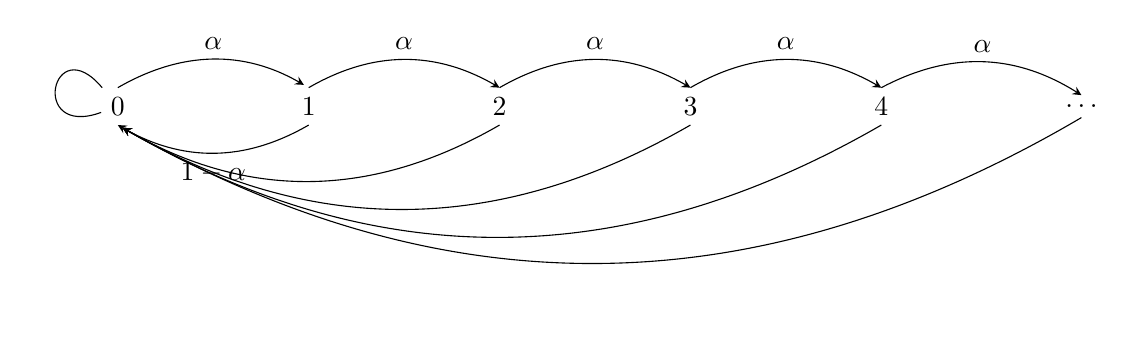
\begin{tikzpicture}
              \node (a) {0};
              \node[right=2cm of a] (b) {1};
              \node[right=2cm of b] (c) {2};
              \node[right=2cm of c] (d) {3};
              \node[right=2cm of d] (e) {4};
              \node[right=2cm of e] (f) {$\ldots$};
            
              \draw (a) to [out=130,in=200,looseness=8] (a);
              %a>b
              \draw[-stealth,shorten >= 2pt] (a.north) to[bend left] node[midway,above] {$\alpha$} (b.north);
              
              %b>c
              \draw[-stealth] (b.north) to[bend left] node[midway,above] {$\alpha$} (c.north);
              \draw[-stealth] (c.north) to[bend left] node[midway,above] {$\alpha$} (d.north);
              \draw[-stealth] (d.north) to[bend left] node[midway,above] {$\alpha$} (e.north);
              \draw[-stealth] (e.north) to[bend left] node[midway,above] {$\alpha$} (f.north);
            
              %b>a
              \draw[-stealth] (b.south) to[bend left] node[midway,below] {$1-\alpha$} (a.south);
              \draw[-stealth,shorten >= 2pt] (d.south) to[bend left] node[midway,below] {} (a.south);
              \draw[-stealth,shorten >= 2pt] (e.south) to[bend left] node[midway,below] {} (a.south);
              \draw[-stealth,shorten >= 2pt] (f.south) to[bend left] node[midway,below] {} (a.south);
              \draw[-stealth,shorten >= 2pt] (c.south) to[bend left] node[midway,below] {} (a.south);
            \end{tikzpicture}
            $$
    Since the chain is irreducible, all states are recurrent.
    
    \newpage 
    \item Find the invariant distribution or determine that one does not exist. If you propose
    an invariant distribution, check that the probabilities add up to 1. Is it a familiar probability distribution with a name?\\
    
    $$
    \begin{pmatrix}
        \pi_0&\pi_1&\pi_2&\pi_3&\ldots
    \end{pmatrix}
    =
    \begin{pmatrix}
        \pi_0&\pi_1&\pi_2&\pi_3&\ldots
    \end{pmatrix}
    \begin{pmatrix}
        1-\alpha&\alpha&0&0&\ldots\\
        1-\alpha&0&\alpha&0&\ldots\\
        1-\alpha&0&0&\alpha&\ldots\\
        \vdots&\vdots&\vdots&\ddots
    \end{pmatrix}
    $$
    
    \begin{itemize}
        \item $\pi_0 = \sum_{k=0}^n  (1-\alpha)\pi_k
        = (1-\alpha)\pi_0 + \sum_{k=1}^n (1-\alpha)\pi_k  $
        
        \item If there exists an invariant distribution, $\sum_{k=0}^n  (1-\alpha)\pi_k = 1$.
        
        \item i.e. $\sum_{k=1}^n (1-\alpha)\pi_k = 1 - \pi_0$
        
        \item So $\pi_0 = \sum_{k=0}^n  (1-\alpha)\pi_k
        = (1-\alpha)\pi_0 + (1-\pi_0)
        = 1 - \alpha$
    \end{itemize}
    Further
    
    \begin{tasks}(2)
        \task $\pi_1 = \alpha\pi_0 = \alpha(1-\alpha)$
        \task $\pi_2 = \alpha(\alpha(1-\alpha))
        = \alpha^2 (1-\alpha)$
    \end{tasks}
    
    Hence we can deduce $\pi_k = \alpha^k (1-\alpha)$ by induction.\\
    
    Thus we can see that the sum of all $\pi_k$ goes to 1.
    $$
    \sum_{k=0}^n \alpha^k(1-\alpha) = \frac{1}{1-\alpha} \cdot (1-\alpha) = 1
    $$
    \newpage
    \item Change the model slightly. Let $0<\beta<1$ be another parameter and suppose that
    immediately after a miss, the next throw succeeds with probability $\beta$. But as before, after a successful free throw, the next shot succeeds with probability $\alpha$. Find again
    the invariant distribution $\pi$. Find also all the probabilities $P_0(T_0 = k)$ for positive integers $k$. Using these probabilities compute the expectation $E_0[T_0]$. Check that your answers satisfy the identity $1/\pi(0) = E_0[T_0]$ as the theory states.\\
    
\textit{Hint.}You may need to evaluate a series of the type $\sum_{k=1}^\infty kx^{k-1}$ for $|x| < 1$. There are several ways to do this. One goes by $\sum_{k=1}^\infty kx^{k-1} = \sum_{k=1}^\infty \sum_{j=1}^k x^{k-1}$ and switches the
order of summation. Another observes that $\sum_{k=1}^\infty kx^{k-1} = \sum_{k=0}^\infty \frac{d}{dx} x^k = \frac{d}{dx}(\sum_{k=0}^\infty x^k),$ evaluates the series and then differentiates.

    $$
    \begin{pmatrix}
        \pi_0&\pi_1&\pi_2&\pi_3&\ldots
    \end{pmatrix}
    =
    \begin{pmatrix}
        \pi_0&\pi_1&\pi_2&\pi_3&\ldots
    \end{pmatrix}
    \begin{pmatrix}
        1-\beta&\beta&0&0&0&\ldots\\
        1-\alpha&0&\alpha&0&0&\ldots\\
        1-\alpha&0&0&\alpha&0&\ldots\\
        1-\alpha&0&0&0&\alpha&\ldots\\
        \vdots&\vdots&\vdots&\vdots&\vdots&\ddots
    \end{pmatrix}
    $$
    
    \begin{itemize}
        \item $\pi_0 = (1-\beta)\pi_0 + (1-\alpha)\pi_1 + (1-\alpha)\pi_2 + \ldots
        = (1-\beta)\pi_0 + \sum_{k=1}^n (1-\alpha)\pi_k$\\
        $= (1-\beta)\pi_0 + (1-\alpha)(1-\pi_0)$
        \item $\cancel{\pi_0} = \cancel{\pi_0} -\beta\pi_0 + 1 -\pi_0 -\alpha +\alpha\pi_0
        \Leftrightarrow \pi_0 = \frac{1-\alpha}{1-\alpha +\beta}$\\
        
        \item $\pi_1 = \beta\pi_0 = \frac{\beta(1-\alpha)}{1-\alpha + \beta}$
        \item $\pi_2 = \beta\pi_1 = \frac{\alpha\beta(1-\alpha)}{1-\alpha+\beta}$\\
        $\vdots$
        \item $\pi_k = \alpha\pi_{k=1} = \frac{\alpha^{k-1}\beta(1-\alpha)}{1-\alpha+\beta}$
    \end{itemize}
    
    Hence
    $$
    \sum_{k=0}^n \pi_k  
    =\frac{1-\alpha}{1-\alpha +\beta} +\frac{\beta(1-\alpha)}{1-\alpha + \beta}
    +\frac{\alpha\beta(1-\alpha)}{1-\alpha+\beta}
    +\frac{\alpha^2\beta(1-\alpha)}{1-\alpha+\beta}
    +\ldots
    $$
    $$
    = \frac{1-\alpha}{1-\alpha +\beta} 
    + \sum_{k=1}^n \frac{\alpha^{k-1}\beta(1-\alpha)}{1-\alpha+\beta}
    = \frac{1-\alpha}{1-\alpha +\beta} 
    + \frac{\beta}{1-\alpha+\beta}\cdot \sum_{k=1}^n \alpha^{k-1}(1-\alpha)
    $$
    Since we proved $\sum_{k=1}^n \alpha^{k-1}(1-\alpha) = 1$ in (b),
    
    $$
    \frac{1-\alpha}{1-\alpha +\beta} 
    + \frac{\beta}{1-\alpha+\beta} 
    =\frac{1-\alpha+\beta}{1-\alpha+\beta}
    =1
    $$
    
\newpage
\item Imagine that the chain of part (c) has been running for a very long time. What is the
probability that the next two shots succeed?\\
\textit{Hint}. For a sanity check of your answer, see that if $\beta = \alpha$ your answer is consistent with the initial description of the free throws.

\vspace{1.5\baselineskip}

    $$
    \begin{pmatrix}
        \pi_0&\pi_1&\pi_2&\pi_3&\ldots
    \end{pmatrix}
    =
    \begin{pmatrix}
        \pi_0&\pi_1&\pi_2&\pi_3&\ldots
    \end{pmatrix}
    \begin{pmatrix}
        0&\beta&0&0&0&\ldots\\
        0&0&\alpha&0&0&\ldots\\
        0&0&0&\alpha&0&\ldots\\
        0&0&0&0&\alpha&\ldots\\
        \vdots&\vdots&\vdots&\vdots&\vdots&\ddots
    \end{pmatrix}
    $$
    \begin{itemize}
        \item $\pi_0 \cdot \beta\cdot \alpha$
        \item $\pi_1\cdot \alpha\cdot\alpha$
        \item $\pi_2\cdot \alpha\cdot\alpha$
        \item $\pi_3\cdot \alpha\cdot\alpha$\\
        \vdots
        \item $\pi_k\cdot \alpha\cdot\alpha$
    \end{itemize}
    
    $$
    P = \pi_0 \cdot \beta\cdot \alpha +\pi_1\cdot \alpha\cdot\alpha + \pi_2\cdot \alpha\cdot\alpha + \ldots + \pi_k\cdot \alpha\cdot\alpha
    $$
    
    $$
    = \alpha\beta\pi_0 + \alpha^2\sum_{k=1}^n \pi_k
    = \alpha\beta\frac{1-\alpha}{1-\alpha+\beta}
    + \alpha^2 \sum_{k=1}^n \frac{\alpha^{k-1}\beta(1-\alpha)}{1-\alpha+\beta}\\
    $$
    
    $$
    = \alpha\beta\frac{1-\alpha}{1-\alpha+\beta} + \frac{\alpha^2\beta}{1-\alpha+\beta}\cdot \sum_{k=1}^n \alpha^{k-1}(1-\alpha)
    $$
    
    $$
    = \alpha\beta\frac{1-\alpha}{1-\alpha+\beta} + \frac{\alpha^2\beta}{1-\alpha+\beta}
    = \frac{\alpha\beta-\alpha^2\beta}{1-\alpha+\beta} + \frac{\alpha^2\beta}{1-\alpha+\beta}
    = \frac{\alpha\beta}{1-\alpha+\beta}
    $$
    
    
    

\newpage
\item Now suppose that we have parameters $\alpha_0, \alpha_1, \alpha_2,...$ all strictly between 0 and 1, and
we specify that, after $k$ consecutive successes, the next shot succeeds with probability
$\alpha_k$. That is, now the transition probabilities are $p(k,k+1) = \alpha_k,\; p(k,0) = 1 - \alpha_k$. Is
it possible to choose the numbers $\alpha_k \in (0,1)$ so that the MC is transient?

    $$
    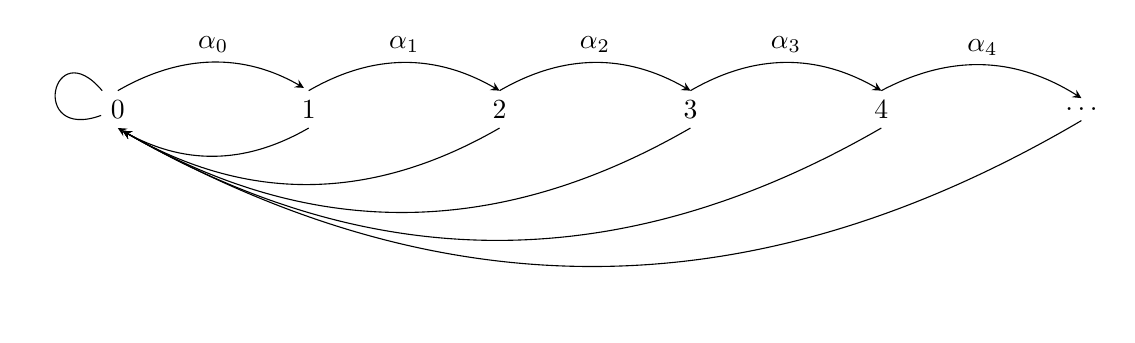
\begin{tikzpicture}
      \node (a) {0};
      \node[right=2cm of a] (b) {1};
      \node[right=2cm of b] (c) {2};
      \node[right=2cm of c] (d) {3};
      \node[right=2cm of d] (e) {4};
      \node[right=2cm of e] (f) {$\ldots$};
    
      \draw (a) to [out=130,in=200,looseness=8] (a);
      %a>b
      \draw[-stealth,shorten >= 2pt] (a.north) to[bend left] node[midway,above] {$\alpha_0$} (b.north);
      \draw[-stealth] (b.north) to[bend left] node[midway,above] {$\alpha_1$} (c.north);
      \draw[-stealth] (c.north) to[bend left] node[midway,above] {$\alpha_2$} (d.north);
      \draw[-stealth] (d.north) to[bend left] node[midway,above] {$\alpha_3$} (e.north);
      \draw[-stealth] (e.north) to[bend left] node[midway,above] {$\alpha_4$} (f.north);
    
      %b>a
      \draw[-stealth] (b.south) to[bend left] node[midway,below] {} (a.south);
      \draw[-stealth,shorten >= 2pt] (d.south) to[bend left] node[midway,below] {} (a.south);
      \draw[-stealth,shorten >= 2pt] (e.south) to[bend left] node[midway,below] {} (a.south);
      \draw[-stealth,shorten >= 2pt] (f.south) to[bend left] node[midway,below] {} (a.south);
      \draw[-stealth,shorten >= 2pt] (c.south) to[bend left] node[midway,below] {} (a.south);
    \end{tikzpicture}
    $$
    
    \begin{itemize}
    \item    Due to its transiency, $p_{00} < 1,\; \text{ so }P_0(T_0 =\infty) = \prod_{k=0}^\infty \alpha_i >$ 0.
    \item Choose $\alpha_k$ such that Markov Chain is transient: $\alpha_k = 1 - \frac{1}{2^k}$.
    \item Then
    $$
    \lim_{n\rightarrow\infty} \prod_{k=0}^\infty\left(1 - \frac{1}{2^k}\right) = \lim_{n\rightarrow\infty} \prod_{k=0}^\infty\left(1 - \frac{1}{2^k}\right)^{\log e = 1} = \lim_{n\rightarrow\infty} e^{\log \prod_{k=0}^\infty\left(1 - \frac{1}{2^k}\right)}
    $$
    
    $$
    =\lim_{n\rightarrow\infty} e^{\log \sum_{k=0}^\infty\left(1 - \frac{1}{2^k}\right)}
    \ge \lim_{n\rightarrow\infty} e^{\log\sum_{k=0}^\infty -\frac{1}{2^k}} > 0
    $$
    \end{itemize}
    
    Thus we proved that there exists such $\alpha_k \in (0,1)$ that the Markov Chain is transient.
    
\newpage
\noindent
\textbf{Question 3}\\
\textbf{Reflected Random Walk.} Fix a parameter $0 < \alpha < 1$. Consider the Markov chain with state space $\mathbb{Z}_{\ge 0} = \{0,1,2,3,...\}$ and transition probability.
$$
p(0,0) = 1 - \alpha, p(x,x+1) = \alpha \text{ for } x \ge 0, \text{ and } p(x,x-1) = 1 - \alpha \text{ for } x \ge 1.
$$
\begin{enumerate}[label=(\alph*)]
    \item Specify for which values of $\alpha$ there exists an invariant distribution. \\
    Find the invariant
    distribution for those values of $\alpha$ for which it exists. 
    
            $$
            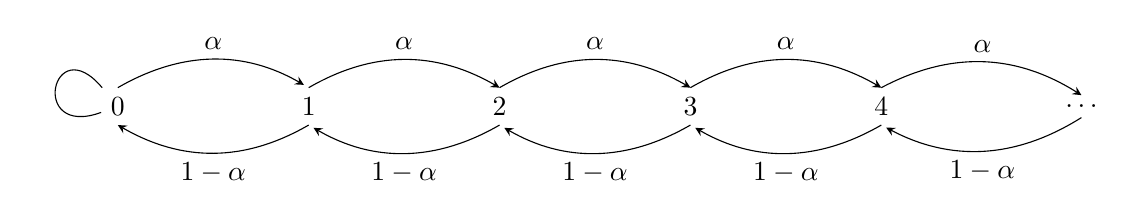
\begin{tikzpicture}
              \node (a) {0};
              \node[right=2cm of a] (b) {1};
              \node[right=2cm of b] (c) {2};
              \node[right=2cm of c] (d) {3};
              \node[right=2cm of d] (e) {4};
              \node[right=2cm of e] (f) {$\ldots$};
            
              \draw (a) to [out=130,in=200,looseness=8] (a);
              %a>b
              \draw[-stealth,shorten >= 2pt] (a.north) to[bend left] node[midway,above] {$\alpha$} (b.north);
              
              %b>c
              \draw[-stealth] (b.north) to[bend left] node[midway,above] {$\alpha$} (c.north);
              \draw[-stealth] (c.north) to[bend left] node[midway,above] {$\alpha$} (d.north);
              \draw[-stealth] (d.north) to[bend left] node[midway,above] {$\alpha$} (e.north);
              \draw[-stealth] (e.north) to[bend left] node[midway,above] {$\alpha$} (f.north);
            
              %b>a
              \draw[-stealth] (b.south) to[bend left] node[midway,below] {$1-\alpha$} (a.south);
              
              %c>b
              \draw[-stealth,shorten >= 2pt] (d.south) to[bend left] node[midway,below] {$1-\alpha$} (c.south);
              \draw[-stealth,shorten >= 2pt] (e.south) to[bend left] node[midway,below] {$1-\alpha$} (d.south);
              \draw[-stealth,shorten >= 2pt] (f.south) to[bend left] node[midway,below] {$1-\alpha$} (e.south);
              \draw[-stealth,shorten >= 2pt] (c.south) to[bend left] node[midway,below] {$1-\alpha$} (b.south);
            \end{tikzpicture}
            $$
    
    $$
        \begin{pmatrix}
            \pi_0&\pi_1&\pi_2&\ldots
        \end{pmatrix}
         = 
        \begin{pmatrix}
            \pi_0&\pi_1&\pi_2&\ldots
        \end{pmatrix}
        \begin{pmatrix}
            1-\alpha&\alpha&0&0&\ldots\\
            1-\alpha&0&\alpha&0&\ldots\\
            0&1-\alpha&0&\alpha&\ldots\\
            0&0&1-\alpha&0&\ldots\\
            0&0&0&1-\alpha&\ldots\\
            \vdots&\vdots&\vdots&\vdots&\ddots\\
            \vdots&\vdots&\vdots&\vdots&\ddots\\
            \vdots&\vdots&\vdots&\vdots&\ddots\\
        \end{pmatrix}
    $$

    \begin{tasks}(2)
        \task $\pi_0 = (1-\alpha)\pi_0 + (1-\alpha)\pi_1$\\
        =\pi_0 - \alpha\pi_0 +\pi_1 - \alpha\pi_1\\
        \Leftrightarrow \pi_0 = \frac{(1-\alpha)\pi_1}{\alpha}
        
        \task \pi_1 = \alpha\pi_0 + (1-\alpha)\pi_2\\
        =\cancel{\alpha}\cdot \frac{(1-\alpha)\pi_1}{\cancel{\alpha}} + (1-\alpha)\pi_2 \\
        \Leftrightarrow \pi_1(1-(1-\alpha)) = (1-\alpha)\pi_2\\
        \Leftrightarrow \pi_1 = \frac{1-\alpha}{\alpha}\pi_2
    \end{tasks}
    
    \vspace{1.5\baselineskip}

    By induction, we obtain $\pi_n = \frac{1-\alpha}{\alpha}\pi_{n+1} = (\frac{\alpha}{1-\alpha})^n \pi_0$.\\
    
    Hence 
    $$\sum_{n>0}^\infty \left(\frac{\alpha}{1-\alpha} \right)^n \pi_0 = \frac{\pi_0}{1-\frac{\alpha}{1-\alpha}}
    = \frac{\pi_0}{\frac{1-2\alpha}{1-\alpha}} = \frac{(1-\alpha)\pi_0}{1-2\alpha} = 1$$
    
    $$
    \Leftrightarrow \pi_0 = \frac{1-2\alpha}{1-\alpha} \Rightarrow \pi_n = \left(\frac{\alpha}{1-\alpha}\right)^n \left(\frac{1-2\alpha}{1-\alpha}\right)
    $$
    
    
    \newpage        
    \item For which values of $\alpha$ is the MC recurrent and for which values transient? Here you probably cannot give a rigorous proof, but you should be able to give an intuitively plausible argument. Note that when you are away from the origin, the reflected random walk behaves just like ordinary random walk.\\
    
    \begin{enumerate}[label=(\roman*)]
        \item $\alpha < 1/2$\\
        As $\alpha$ gets smaller, it is more probable to come back to 0. However this recurrence is finite, so we can consider this to be a positive recurrent case.
        
        \item $\alpha = 1/2$\\
        In case of $\alpha = \frac{1}{2}$, recurrence will be occurred infinitely many times (null-recurrence). It is always coming back to 0.
        
        \item $\alpha > 1/2$\\
        As $\alpha$ gets larger, it is more probable to go forward, which is transient.

        
    \end{enumerate}
\end{enumerate}


\newpage
\noindent 
\textbf{Question 4}\\
\textbf{Symmetric Simple Random Walk.} Consider the Markov chain with state space $S = \mathbb{Z} = \{...,-2,-1,0,1,2,...\}.$ The transition probabilities for this chain are
$$
p(j,j-1) = \frac{1}{2}, p(j,j+1) = \frac{1}{2}
$$
for all $j\in S$. Find all the stationary measures and stationary distributions for this Markov
chain.

            $$
            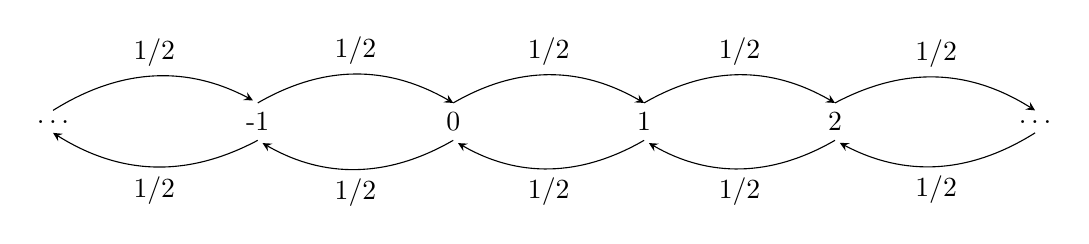
\begin{tikzpicture}
              \node (a) {$\ldots$};
              \node[right=2cm of a] (b) {-1};
              \node[right=2cm of b] (c) {0};
              \node[right=2cm of c] (d) {1};
              \node[right=2cm of d] (e) {2};
              \node[right=2cm of e] (f) {$\ldots$};
            
              %a>b
              \draw[-stealth,shorten >= 2pt] (a.north) to[bend left] node[midway,above] {1/2} (b.north);
              
              %b>c
              \draw[-stealth] (b.north) to[bend left] node[midway,above] {1/2} (c.north);
              \draw[-stealth] (c.north) to[bend left] node[midway,above] {1/2} (d.north);
              \draw[-stealth] (d.north) to[bend left] node[midway,above] {1/2} (e.north);
              \draw[-stealth] (e.north) to[bend left] node[midway,above] {1/2} (f.north);
            
              %b>a
              \draw[-stealth] (b.south) to[bend left] node[midway,below] {1/2} (a.south);
              
              %c>b
              \draw[-stealth,shorten >= 2pt] (d.south) to[bend left] node[midway,below] {1/2} (c.south);
              \draw[-stealth,shorten >= 2pt] (e.south) to[bend left] node[midway,below] {1/2} (d.south);
              \draw[-stealth,shorten >= 2pt] (f.south) to[bend left] node[midway,below] {1/2} (e.south);
              \draw[-stealth,shorten >= 2pt] (c.south) to[bend left] node[midway,below] {1/2} (b.south);
            \end{tikzpicture}
            $$
            
    $$
    \begin{pmatrix}
        \pi_1&\pi_2&\pi_3&\ldots
    \end{pmatrix}
    = 
    \begin{pmatrix}
        \pi_1&\pi_2&\pi_3&\ldots
    \end{pmatrix}
    \begin{pmatrix}
              &\ldots&\ldots&\ldots&\ldots&\ldots&\ldots&\vdots\\
        \vdots&\ddots&\ldots&\ldots&\ldots&\ldots&\ldots&\vdots\\
        \vdots&\ldots&1/2&0&1/2&\ldots&\ldots&\vdots\\
        \vdots&\ldots&\ldots&1/2&0&1/2&\ldots&\vdots&\\
        \vdots&\ldots&\ldots&\ldots&1/2&0&1/2&\vdots\\
        \vdots&\ldots&\ldots&\ldots&\ldots&\ddots&0&\vdots\\
        \vdots&\ldots&\ldots&\ldots&\ldots&\ldots&\ddots&\vdots\\
    \end{pmatrix}
    $$
    
    $$
    \Rightarrow \pi_k = \frac{1}{2}\pi_{k-1}+\frac{1}{2}\pi_{k+1}
    \Leftrightarrow 2\pi_k = \pi_{k-1}+\pi_{k+1} 
    \Leftrightarrow \pi_{k+1} - \pi_k = \pi_k - \pi_{k-1}
    $$
    
    Since this is an arithmetic sequence which has same difference between adjacent terms, $\pi_k$ can be expressed as $\pi_k = a + bk$.\\
    
    Since $\pi_k$ should be non-negative, $b =0$. However, then, $\sum_{k=0}^n \pi_k$ does not have to be 0. Thus it diverges and there does not exist a stationary distribution for the symmetric simple random walk.
    
    
\end{enumerate}

\newpage
\noindent 
\textbf{Exercise 1.13} Consider the Markov chain with transition matrix:
$$
\begin{matrix}
    &1&2&3&4\\
    \textbf{1}&0&0&0.1&0.9\\
    \textbf{2}&0&0&0.6&0.4\\
    \textbf{3}&0.8&0.2&0&0\\
    \textbf{4}&0.4&0.6&0&0
\end{matrix}
$$
\begin{enumerate}[label=(\alph*)]
    \item Compute $p^2$.
    $$ p^2 =
    \begin{bmatrix}
        0&0&0.1&0.9\\
        0&0&0.6&0.4\\
        0.8&0.2&0&0\\
        0.4&0.6&0&0
    \end{bmatrix}
    \cdot 
    \begin{bmatrix}
        0&0&0.1&0.9\\
        0&0&0.6&0.4\\
        0.8&0.2&0&0\\
        0.4&0.6&0&0
    \end{bmatrix}
    =
    \begin{bmatrix}
        0.44&0.56&0&0\\
        0.64&0.36&0&0\\
        0&0&0.2&0.8\\
        0&0&0.4&0.6
    \end{bmatrix}
    $$
    \item Find the stationary distributions of $p$ and all of the stationary distributions of $p^2$.
    
        \begin{itemize}
            \item The stationary distribution of $p$.\\
            $$
             \begin{bmatrix}
                \pi_1&\pi_2&\pi_3&\pi_4\\
            \end{bmatrix}
            \cdot 
            \begin{bmatrix}
                0&0&0.1&0.9\\
                0&0&0.6&0.4\\
                0.8&0.2&0&0\\
                0.4&0.6&0&0
            \end{bmatrix}
            =
            \begin{bmatrix}
                \pi_1&\pi_2&\pi_3&\pi_4\\
            \end{bmatrix}   
            $$
            
            \begin{tasks}(2)
        		\task $0.8\pi_3 + 0.4\pi_4 = \pi_1$
        		\task $0.2\pi_3 + 0.6\pi_4 = \pi_2$
        		\task $0.1\pi_1 + 0.6\pi_2 = \pi_3$
        		\task $0.9\pi_1 + 0.4\pi_2 = \pi_4$
        		
        	\end{tasks}
            
            Hence, we obtain following equations.
            $$\pi_1+\pi_2 = \pi_3+\pi_4 = \frac{1}{2}$$
            
            Then (ii) + (iii)
            $$\pi_2 + \pi_3 = 0.1\pi_1 + 0.6\pi_2 + 0.2\pi_3 + 0.6\pi_4$$
            $$0.4\pi_2 + 0.8\pi_3 = 0.1\pi_1 + 0.6\pi_4$$
            $$0.4(0.2\pi_3 + 0.6\pi_4) + 0.8\pi_3 = 0.1(0.8\pi_3 + 0.4\pi_4) + 0.6\pi_4$$
            $$\cancel{0.08\pi_3} + 0.24\pi_4 + 0.8\pi_3 = \cancel{0.08\pi_3} + 0.04\pi_4 + 0.6\pi_4$$
            $$0.24\pi_4 + 0.8\pi_3 = 0.64\pi_4 \Leftrightarrow 0.8\pi_3 = 0.4\pi_4 
            \Leftrightarrow 2\pi_3 = \pi_4$$
            
            Plugging $2\pi_3 = \pi_4$ into (i) and (ii),
            $$0.8\pi_3 + 0.8\pi_3 = 1.6\pi_3 = \pi_1 \qquad
            0.2\pi_3+1.2\pi_3 = 1.4\pi_3 = \pi_2
            $$
            Thus the stationary distribution of $p$ is
            $$\pi = \left[ \frac{4}{15}\quad \frac{7}{30}\quad \frac{1}{6}\quad \frac{1}{3} \right] $$
            \newpage
            \item The stationary distribution of $p^2$.\\
            
            $$
            \begin{bmatrix}
                \pi_1&\pi_2&\pi_3&\pi_4\\
            \end{bmatrix}
            \cdot 
            \begin{bmatrix}
                0.44&0.56&0&0\\
                0.64&0.36&0&0\\
                0&0&0.2&0.8\\
                0&0&0.4&0.6
            \end{bmatrix}
            =
            \begin{bmatrix}
                \pi_1&\pi_2&\pi_3&\pi_4\\
            \end{bmatrix}   
            $$
            \begin{tasks}(2)
        		\task $0.44\pi_1 + 0.64\pi_2 = \pi_1$
        		\task $0.56\pi_1 + 0.36\pi_2 = \pi_2$
        		\task $0.2\pi_3 + 0.4\pi_4 = \pi_3$
        		\task $0.8\pi_3 + 0.6\pi_4 = \pi_4$
        	\end{tasks}
        
        
            Hence, we obtain following equations.
        
            $$0.56\pi_1 = 0.64\pi_2 \Longleftrightarrow \pi_2 = \frac{7}{8} \pi_1 \qquad
                0.8\pi_3 =0.4\pi_4 \Longleftrightarrow \pi_3 = \frac{1}{2}\pi_4$$
            
            $$\pi_1+\pi_2+\pi_3+\pi_4 = \frac{15}{8} \pi_1 + 3\pi_3 = 1
            $$
            Thus the stationary distribution is
            $$\pi = \left[\pi_1\quad \frac{7}{8}\pi_1\quad \frac{1-\frac{15}{8}\pi_1}{3}\quad \frac{2(1-\frac{15}{8}\pi_1)}{3}  \right] $$
        \end{itemize}
    
    \item Find the limit of $p^{2n} (x,x)$ as $n \rightarrow \infty.$
    
    To find the limit, we have to use the irreducible recurrent classes.\\
    For states $\{1,2\}$ in the upper-left part of the matrix,
    \begin{itemize}
        \item $\lim\limits_{n\to\infty}p^{2n}(1,1) = \pi^1(1)=8/15$
        \item $\lim\limits_{n\to\infty}p^{2n}(2,2) = \pi^1(2)=7/15$
    \end{itemize}
    
    For states $\{1,2\}$ in the lower-right part of the matrix,
    \begin{itemize}
        \item $\lim\limits_{n\to\infty}p^{2n}(3,3) = \pi^2(3)=1/3$
        \item $\lim\limits_{n\to\infty}p^{2n}(4,4) = \pi^2(4)=2/3$
    \end{itemize}
    

    $$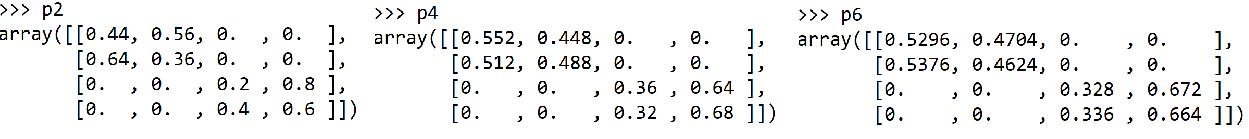
\includegraphics[width=\textwidth]{hw3_np1.png}$$
    $$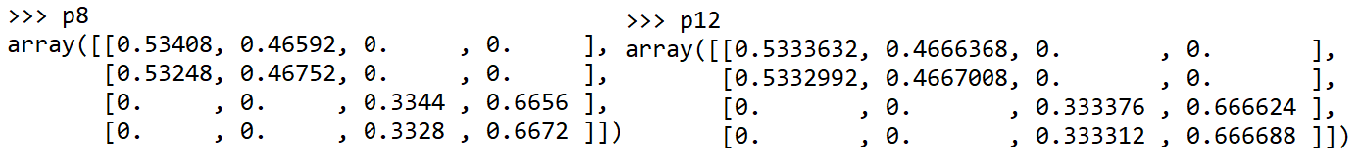
\includegraphics[width=\textwidth]{hw3_np2.png}$$
    
    Calculating the matrix multiplication through Python (pi = $p^i$ where $i = \mathbb{Z}_{2,4,6,...}$)\\ 
    also found that, as $n \rightarrow \infty$, $p^{2n} (x,x)$ converges to 
    
    $$
    \begin{bmatrix}
        8/15&7/15&0&0\\
        8/15&7/15&0&0\\
        0&0&1/3&2/3\\
        0&0&1/3&2/3
    \end{bmatrix}
    $$
\end{enumerate}


\newpage
\noindent 
\textbf{Exercise 1.32}
The weather in a certain town is classified as rainy, cloudy, or sunny and
changes according to the following transition probability is

$$
\begin{matrix}
    &\textbf{R}&\textbf{C}&\textbf{S}\\
    \textbf{R}&1/2&1/4&1/4\\
    \textbf{C}&1/4&1/2&1/4\\
    \textbf{S}&1/2&1/2&0
\end{matrix}
$$




In the long run what proportion of days in this town are rainy? cloudy? sunny?\\
\vspace{1.5\baselineskip}

This chain is aperiodic, closed irreducible.  i.e. $p^n(x,y) \xrightarrow[\text{$n\rightarrow \infty$}]{}   \pi(y)\;\;\forall\; x,y\in S $\\
Hence the convergence theorem is needed to find its stationary distribution.

$$
\begin{pmatrix}
    \pi_1&\pi_2&\pi_3 
\end{pmatrix}
\begin{pmatrix}
    1/2&1/4&1/4\\
    1/4&1/2&1/4\\
    1/2&1/2&0
\end{pmatrix}
=
\begin{pmatrix}
    \pi_1&\pi_2&\pi_3 
\end{pmatrix}
$$
\vspace{1.5\baselineskip}
\begin{align}
    \frac{1}{2}\pi_1 + \frac{1}{4}\pi_2 + \frac{1}{2}\pi_3 = \pi_1\\
    \frac{1}{4}\pi_1 + \frac{1}{2}\pi_2 + \frac{1}{2}\pi_3 = \pi_2\\
    \frac{1}{4}\pi_1 + \frac{1}{4}\pi_2 \qquad\quad = \pi_3
\end{align}
Plugging (3) into (2)
$$
\frac{1}{2}\pi_1 + \frac{1}{4}\pi_2 +\frac{1}{2}\left(\frac{1}{4}(\pi_1+\pi_2)
\right)
= \left(\frac{1}{2} + \frac{1}{8} \right)\pi_1 + \left(\frac{1}{4} + \frac{1}{8}\right)\pi_2
$$
$$
= \frac{5}{8}\pi_1 + \frac{3}{8}\pi_2 = \pi_2 
\Leftrightarrow \pi_1 = \pi_2
$$
Hence in (3),
$$
\frac{1}{4}\pi_1 + \frac{1}{4}\pi_2 = \frac{1}{2}\pi_1 = \pi_3
\Leftrightarrow \pi_1 = 2\pi_3
$$
Finally
$$
\pi_1+\pi_2+\pi_3 = 1 \Leftrightarrow 2\pi_3 + 2\pi_3 + \pi_3 = 5\pi_3 = 1
$$
$$
\Leftrightarrow \pi_3 = \frac{1}{5}, \text{ so } \pi_1=\pi_2 = \frac{2}{5}
$$

$$
\pi = 
\begin{pmatrix}
    \frac{2}{5}&\frac{2}{5}&\frac{1}{5}
\end{pmatrix}
$$

\end{document}